
%\documentclass{svjour3}                     % onecolumn (standard format)
%\documentclass[smallcondensed]{svjour3}     % onecolumn (ditto)
\documentclass[12pt,oneside,a4paper]{article}  

\usepackage{apacite}
\usepackage{appendix}
\usepackage{amsmath}
\usepackage{amsthm}

\usepackage{amssymb} % for approx greater than
\usepackage{caption}
\usepackage{placeins} % for \FloatBarrier
\usepackage{graphicx}
%\usepackage{subcaption}
\usepackage{longtable}
\usepackage{setspace}
\usepackage{booktabs}
\usepackage{tabularx}
\usepackage{xcolor,colortbl}
\usepackage{chngpage}
\usepackage{natbib}
\bibpunct{(}{)}{,}{a}{}{;} 
\usepackage{url}
\usepackage{nth}
\usepackage{authblk}
\usepackage[most]{tcolorbox}
\usepackage[normalem]{ulem}
\usepackage{amsfonts}
%\smartqed  
% columns for longtable
\usepackage{arydshln} % Dashed lines in matrices

\usepackage[margin=1in]{geometry}
%\doublespacing % for review
\newcommand{\absdiv}[1]{%
  \par\addvspace{.5\baselineskip}% adjust to suit
  \noindent\textbf{#1}\quad\ignorespaces
}

% line numbers to make review easier
%\usepackage{lineno}
%\linenumbers

%\usepackage{soul}% for \st{}

%%%%%%%%%%%%%%%%%%%%%%%%%%%%%%%%%%%%%%%%%%%%%%%%%%%%%%%%%%%%%%%%%%%%%%%%%%%%%%
% for section 4 math environments
\theoremstyle{definition}
\newtheorem{definition}{Definition}[section]
\newtheorem{theorem}{Theorem}[section]
\newtheorem{proposition}{Proposition}[section]
\newtheorem{corollary}{Corollary}[proposition]
\newtheorem{remark}{Remark}[section]
%

%\end{filecontents*}
%\RequirePackage{fix-cm}

% \newcommand\ackn[1]{%
%   \begingroup
%   \renewcommand\thefootnote{}\footnote{#1}%
%   \addtocounter{footnote}{-1}%
%   \endgroup
% }

% Affiliations in small font size
%\renewcommand\Affilfont{\small}
\usepackage{tcolorbox}
\defcitealias{HMD}{HMD 2016}

% junk for longtable caption
%\AtBeginEnvironment{longtable}{\linespread{1}\selectfont}
%\setlength{\LTcapwidth}{\linewidth}

% sort van Raalte properly
% #1: sorting key, #2: prefix for citation, #3: prefix for bibliography
%\DeclareRobustCommand{\VAN}[3]{#2} % set up for citation
\newcommand{\tc}{\quad\quad\text{,}}
\newcommand{\tp}{\quad\quad\text{.}}
\newcommand{\vb}[1]{\texttt{#1}}
%%%%%%%%%%%%%%%%%%%%%%%%%%%%%%%
\begin{document}


\title{Time spent and left of transient states in
stationary populations}

\author[1]{Tim Riffe\thanks{riffe@demogr.mpg.de}}
\author[2]{Francisco Villavicencio}
\author[3]{Nicolas Brouard}

\affil[1]{Max-Planck-Institute for Demographic Research}
\affil[2]{University of Southern Denmark}
\affil[3]{Institut National d'\'Etudes D\'emographiques}



%\authorrunning{Short form of author list} % if too long for running head

\maketitle

\vspace{-2em}
%\begin{abstract}
%\authorrunning{Short form of author list} % if too long for running head

% \institute{   Tim Riffe \at
%               Max Planck Institute for Demographic Research.
%               Konrad-Zuse-Str. 1. 18057 Rostock, Germany\\
%               \email{riffe@demogr.mpg.de}\\
%               Tel.:  +49 176 232 858 45\\
%               Fax: +49 381 2081 - 280
% \and 
% Francisco Villavicencio \at
%               Department of Public Health \& Max-Planck Odense Center on the
%               Biodemography of Aging. University of Southern Denmark, J.B. Winsl?ws Vej 9B, 
%               2nd floor DK-5000 Odense C, Denmark \\
%               \email{fvillavicencio@health.sdu.dk}
%               }
              
%\journalname{Demographic Research}
%\date{Received: date / Accepted: date}
\maketitle

\begin{abstract}
\absdiv{Background} The Brouard-Carey equality establishes equality
between the distributions of years-lived and years-left in stationary populations. 
\absdiv{Objective} We aim to generalize this equality to account for time
spent and time left in states within multistate stationary populations. 
\absdiv{Results} We
provide two intuitive proofs that the distribution of time spent and left in
transient states is equal in multistate stationary populations.
\absdiv{Conclusions} This equality may be helpful under
certain constraints to estimate the distribution of otherwise unobserved onset timing for health or other states.
%\keywords{Brouard-Carey equality \and Stationary population \and Age
%structure \and Symmetric patterns \and Multistate models}
%\subclass{91D20 \and 60K05 \and 92D25}
\end{abstract}

\section{Background}
The Brouard-Carey equality establishes that the distributions of years-lived and years-left are identical in perfectly stationary populations
\citep{brouard1989mouvements,Vaupel2009,rao2014,villavicencioRiffeSymmetires2016}. Consider the case of multistate stationary populations, as implied by fixed transition rate schedules (over age) that govern mortality and the movement of individuals between a finite number of states. Multistate stationary populations are characterized by a fixed age-state structure \citep{perron1907theorie,frobenius1912matrizen}, a property often exploited by Markov
models with the goal of estimating state expectancies or similar. Since the age-state distribution is a fixed attribute, summing over states within age produces an age distribution that is also a fixed attribute, and it follows that the Brouard-Carey equality still holds in the aggregate with respect to age and remaining years of life distributions. 

Individual discrete lifecourse trajectories resulting from fixed transition rate schedules consist in sequences of states. Such trajectories are not completely random processes, but these are constrained in the limit to abide by the laws of probability. Specifically, the probability of observing any particular discrete lifecourse trajectory (Markov sampling path) is the product of the sequence of transition probabilities required to produce it. If mortality probabilities close out with 1, then the sum of the probabilities of all possible trajectories is one. The set of all possible trajectories (and their corresponding probabilities of occurring) --- a potentially very large set of distinct trajectories --- is also a fixed attribute of the stationary population. 

Throughout this exposition we rely on the notion of a multistate stationary population; we therefore first offer a toy example of one to illustrate some of the properties that form the background to the symmetry property that we wish to describe. Define a two-state model of healthy (\vb{H}) and sick (\vb{S}) with three age classes, and including bidirectional flows between states as well as exits from each state to death (\vb{D}). A set of example transition rates are given in Tab.~\ref{tab:toy}. Each new birth also has a .9 (.1) probability of being born healthy (sick). 
% latex table generated in R 3.4.0 by xtable 1.8-2 package
% Wed Apr  4 13:28:00 2018
% \begin{table}[ht]
% \caption{Example transition rates in three discrete age classes for transitions within and between good health (\vb{H}) and sickness (\vb{S}), and to death (\vb{D}).}
% \label{tab:toy}
% \centering
% \begin{tabular}{rrrrrrr}
%   \hline
% Age class& \vb{H}$\rightarrow$\vb{H} & \vb{H}$\rightarrow$\vb{S} & \vb{H}$\rightarrow$\vb{D} & \vb{S}$\rightarrow$\vb{S} & \vb{S}$\rightarrow$\vb{H} & \vb{S}$\rightarrow$\vb{D} \\ 
%   \hline
% 1 & 0.89 & 0.10 & 0.01 & 0.10 & 0.70 & 0.20 \\ 
%   2 & 0.70 & 0.20 & 0.10 & 0.20 & 0.50 & 0.30 \\ 
%   3 & 0.00 & 0.00 & 1.00 & 0.00 & 0.00 & 1.00 \\ 
%    \hline
% \end{tabular}\end{table}


% latex table generated in R 3.4.0 by xtable 1.8-2 package
% Mon Apr 16 11:31:53 2018
\begin{table}[ht]
\centering
 \caption{Example transition rates in four discrete single age classes for transitions within and between good health (\vb{H}) and sickness (\vb{S}), and to death (\vb{D}).}
 \label{tab:toy}
\begin{tabular}{rrrrrrr}
  \hline
Age & HH & HS & HD & SS & SH & SD \\ 
  \hline
0 & 0.89 & 0.10 & 0.01 & 0.10 & 0.70 & 0.20 \\ 
  1 & 0.70 & 0.20 & 0.10 & 0.20 & 0.50 & 0.30 \\ 
  2 & 0.50 & 0.30 & 0.20 & 0.30 & 0.30 & 0.40 \\ 
  3 & 0.00 & 0.00 & 1.00 & 0.00 & 0.00 & 1.00 \\ 
   \hline
\end{tabular}
\end{table}

\noindent Hold transition rate schedules fixed for a sufficiently long time, such that strong ergodicity takes hold, and hold the population to a constant size. Each new cohort is expected be identical, and the numbers of healthy and sick individuals in each age are expected to be the same in each time step. The set of potential discrete trajectories that might arise from these transition probabilities, and the probability of observing each, is given in Tab.~\ref{tab:traj}:

% latex table generated in R 3.4.0 by xtable 1.8-2 package
% Wed Apr  4 13:50:17 2018
% \begin{table}[ht]
% \caption{The set of all possible discrete trajectories and probability of observing each, given the transition rates in Tab.~\ref{tab:toy}. }
% \label{tab:traj}
% \centering
% \begin{tabular}{lr}
%   \hline
% Trajectory & Probability \\ 
%   \hline
% \vb{H} & 0.0090 \\ 
%   \vb{S} & 0.0200 \\ 
%   \vb{HH} & 0.0801 \\ 
%   \vb{SH} & 0.0070 \\ 
%   \vb{HS} & 0.0270 \\ 
%   \vb{SS} & 0.0030 \\ 
%   \vb{HHH} & 0.5607 \\ 
%   \vb{SHH} & 0.0490 \\ 
%   \vb{HSH} & 0.0450 \\ 
%   \vb{SSH} & 0.0050 \\ 
%   \vb{HHS} & 0.1602 \\ 
%   \vb{SHS} & 0.0140 \\ 
%   \vb{HSS} & 0.0180 \\ 
%   \vb{SSS} & 0.0020 \\ 
%    \hline
%    Total & 1.0000
% \end{tabular}
% \end{table}

% latex table generated in R 3.4.0 by xtable 1.8-2 package
% Mon Apr 16 11:33:28 2018
% latex table generated in R 3.4.0 by xtable 1.8-2 package
% Mon Apr 16 11:35:50 2018
\begin{table}[ht]
\centering
 \caption{The set of all possible discrete transient trajectories and probability of observing each, given the transition rates in Tab.~\ref{tab:toy}. }
 \label{tab:traj}
\begin{tabular}{lc|lc}
  \hline
Trajectory & Probability & Trajectory & Probability \\ 
  \hline
\vb{H} & 0.00900 & \vb{SHHH} & 0.02450 \\ 
  \vb{S} & 0.02000 & \vb{HSHH} & 0.02250 \\ 
  \vb{HH} & 0.08010 & \vb{SSHH} & 0.00250 \\ 
  \vb{SH} & 0.00700 & \vb{HHSH} & 0.04806 \\ 
  \vb{HS} & 0.02700 & \vb{SHSH} & 0.00420 \\ 
  \vb{SS} & 0.00300 & \vb{HSSH} & 0.00540 \\ 
  \vb{HHH} & 0.11214 & \vb{SSSH} & 0.00060 \\ 
  \vb{SHH} & 0.00980 & \vb{HHHS} & 0.16821 \\ 
  \vb{HSH} & 0.00900 & \vb{SHHS} & 0.01470 \\ 
  \vb{SSH} & 0.00100 & \vb{HSHS} & 0.01350 \\ 
  \vb{HHS} & 0.06408 & \vb{SSHS} & 0.00150 \\ 
  \vb{SHS} & 0.00560 & \vb{HHSS} & 0.04806 \\ 
  \vb{HSS} & 0.00720 & \vb{SHSS} & 0.00420 \\ 
  \vb{SSS} & 0.00080 & \vb{HSSS} & 0.00540 \\ 
  \vb{HHHH} & 0.28035 & \vb{SSSS} & 0.00060 \\ 
  \hline
  &&Total& 1.00000\\
   \hline
\end{tabular}
\end{table}

For example, given a birth cohort of 100000 individuals, we would expect to see 900 individuals that are born healthy and then die before reaching the second age class. We can force these proportions to be exact either via deterministic renewal of the population, or as a limiting property as the population size approaches infinity. More ages and states will make the number of potential trajectories factorially larger, but the sum of the probabilities of all trajectories will always be one. The important feature for the present is that the detailed discrete lifecourse composition of each entering cohort is under these conditions identical, uniquely defined by the transition rates, and therefore a feature of the multistate stationary population. By extension, the composition by state episodes (with respect to e.g. episode duration and timing) is identical under stationarity. This property forms the groundwork to the proof of our main result.

%A perfectly stationary population is either \emph{perfectly} stationary because it is
%of infinite size, because it is finite and
%deterministically repeating, or as a time-invariant expectation resulting from fixed vital rates. Whether vital rates are treated as generative (traditional) or artifactual, rate schedules must be fixed and the intrinsic growth rate constant at null.
% NB: remove fertility. Define multistate stationary in a more direct a rigorous way
% as arising from fixed age-specific force of transition and mortality. No need
% to speak of fertiltiy.
% Let's say that individuals in
% the stationary population can obtain different states over the life course. If
% birth and death rates do not vary by states, then it does not matter whether
% state transition rates are fixed or not, for in the aggregate the population remains
% stationary in the traditional sense. However, if vital rates depend on one's
% state, transition rates must also be fixed in order for stationarity to
% hold in the aggregate--- This is the situation that we entertain in the
% following. Under fixed vital and state-transition rates, where vital rate
% schedules differ between states, the standard set of aggregate invariant
% quantities of course remains:
% birth cohorts and death cohorts are of fixed and equal size. 
% Further, the
% Brouard-Carey equality still holds in the aggregate. 
% Under these conditions,
% once stationarity is achieved, the age-state structure of the stationary
% population is also invariant over time
%, a property often exploited by Markov
%models where the goal is to estimate state expectancies or similar. 
% As a
% consequence of fixed transition and vital rate schedules, the distribution of state-specific tenures for individuals entering a state at a given age is also a fixed attribute: These are mereley aggregations over individuals, and the probability of any particular life course trajectory is also fixed.

% This setup is not entirely contrived, for it corresponds with the assumptions of
% common multistate markov models, often used to calculate state expectancies.
% In the present, however, we are not bound to memoryless transition probabilities.
% Instead, we simply require the consequence of (or the expectation of) invariant
% age-state structure and invariant conditional age-state tenure distributions, which may result from
% either memoryless transitions, or from arbitrarily linked
% dependencies.
% It is the fact of fixed age-state flows and structure on which we base the following observations.
% In essence, the population consists in set of lives that is a fixed distribution of lifecourse
% trajectories, each consisting in a sequence of discrete state-specific
% durations. This set could be of infinite size (but discrete time intervals), in
% which case the fraction of births destined to live a given trajectory is fixed,
% or it could exist as a fixed occurrence probability (the product of
% transition probabilities required to live said trajectory). 
% 
% Under fixed vital and transition rates, and zero growth, 
\section{Relationship}
We introduce an extension of the Brouard-Carey equality to states in multistate stationary populations.
Formally:

% NB: change to language of x+delta x, or change to census at time t
% the probability of being < x years in state (or state 0-x years).
% same as remaining in state for at most another x years. Or something like this.
% discretize the theorem. 
\begin{theorem}
\label{th}
Given a multistate stationary population that has been stationary for a suffiently long time, the probability that an individual randomly selected at time $t$ is in state $s$ and has been in $s$ continuously for at least $x$ time is equal to the probability of being in state $s$ and remaining in $s$ for at least $x$ time.
\end{theorem}

Equivalently, the distribution of time spent in $s$ is equal to the distribution of time left in $s$. This proposition
might not be intuitive at first glance, so we prove it, and then speculate
as to how this equality may be put to good use. 


\section{Two proofs of within-state symmetry}
\FloatBarrier

We provide two discrete proofs of theorem~\ref{th}. Each may appeal to a differnt kind of intuition. The first is built up from the possible discrete life trajectories defined by a set of transition probabilities, such as those shown in Tab.~\ref{tab:traj}. The second follows the Lexis aggregate approach of \citet{villavicencioRiffeSymmetires2016}.

\begin{proof}[Proof 1 of Theorem \ref{th}]
This proof follows four steps, which we illustrate and interleave with a worked example based on the transition rates in Tab.~\ref{tab:toy}:
\begin{enumerate}
\item{\textbf{Complementarity identity:}} The lengths of two durations created by bisection of a single continuous duration sum to the length of the original duration. A duration can be represented as a line segment, potentially representing a state episode that comprises a subsection of a life-line. Points along a single within-person duration can be
sampled over time in arbitrarily fine and regular time steps, $\delta$. Each
time step is a segment bisector, collecting two sets of
values: 1) time spent in the state prior to the sample point, and 2) time
left until exiting the state.
If observations are evenly spaced, and values are truncated to the nearest
$\delta$, by way of complements these two sets will consist of the same values.

If the duration of the $j^{th}$ episode of the $i^{th}$ potential life trajectory is called $d^{i,j}$, the age of entry
is $a_L^{i,j}$ and the age of exit is $a_R^{i,j}$, such that $d^{i,j} = a_R^{i,j} -
a_L^{i,j}$. The set of time-spent values that one would sample over the course of $d^{i,j}$, $A^{i,j}$ is defined as:
\begin{align}
\label{eq:Ai}
A^{i,j} &= \left\{ \delta \cdot k ~| ~k \in \mathbb{Z}^+~, ~0 \le k \le
\left\lfloor \frac{d^{i,j}}{\delta}\right\rfloor \right\} \tc \intertext{where
$\lfloor \ldots\rfloor $ denotes truncation to the lower integer bound. The
set of time left values, $T^i$ is also:}
\label{eq:Ti}
T^i &= \left\{ \delta \cdot k ~| ~k \in \mathbb{Z}^+~, ~\left\lfloor
\frac{d^{i,j}}{\delta}\right\rfloor \ge k \ge 0\right\} \tp
\end{align}
Figure~\ref{fig:lifeline1} illustrates the construction of
$A^{i,j}$ and $T^{i,j}$ in expressions~\eqref{eq:Ai} and \eqref{eq:Ti}. The central bisector moves along the duration from the time of entry until the time of exit, creating two
sets of values.

\begin{figure}[h!]
\centering
\caption{A lifeline of the $j^{th}$ episode of a reference state individual $i$ showing the construction of the sets $A^{i,j}$
and $T^{i,j}$.}
\label{fig:lifeline1}
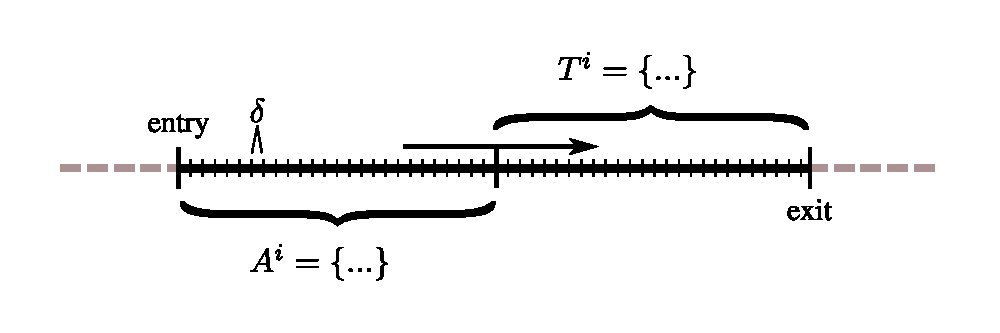
\includegraphics[scale=.8]{Figures/lifeline1.pdf}
\end{figure}

\begin{tcolorbox}
For example, from the \nth{21} life trajectory in Tab.~\ref{tab:traj}, \vb{HSSH}, sickness might be the state of interest, in which case \vb{SS} becomes the episode of interest in this trajectory. If each time step is a year, $\delta = 1$, then we have $A^{21,1} = \{ 0,1,2 \}$ and $T^{21,1} = \{ 2,1,0 \}$: Where order does not matter, these are two equal sets. These figures are predicated on the strict and limiting assumption that the census is on January 1, each cohort is generated on January 1, and 0s (moment of entry or exit) are observed. This implies five observable points in a life passing through four age classes, but it simplifies the example by not having to specify a distribution over intervals.
\end{tcolorbox}



\FloatBarrier
\item{\textbf{Complementarity identity over replicated life trajectories:}} Under stationarity, the probability of generating a given trajectory is replicated every $\delta$ time step, where $\delta$ is the same time step over time and age, i.e., the same spacing as our observation spacing in figure~\ref{fig:lifeline1}) but extended over a
 Lexis space. This can be represented with a set of age-aligned and identically long cohort segments placed side-by-side, spaced apart by $\delta$.
% This potentially large set of segments may be imagined as a plane, although this
% would only hold in the limit.
One could in this setting take a census at a single point in time, collecting a set of
time spent and time left values ($A^{i,j}$ and $T^{i,j}$), each from a repeated episode in
sequence.
The two sets observed at a single time point but drawn from the replicating population of life trajectories will be identical to the first two sets that were sampled from
a single duration over its entire duration, if the same $\delta$-truncation is applied.

Figure~\ref{fig:clones} illustrates this notion with uniformly-spaced lifelines
in a Lexis configuration. The vertical line indicates a hypothetical census at time $t$ of
the population of this replicated life trajectory. At time $t$, the blue-highlighted segments indicate
the set of time-spent values in $A^{i,j}$, and red-highlighted segments are the
time-left elements of $T^{i,j}$. 

 \begin{figure}[h!]
\centering
\caption{The $j^{th}$ episode of the $i^th$ life trajectory is repeated in $\delta$ time steps. A
census with followup now constructs the sets $A^{i,j}$ and $T^{i,j}$ with values
identical to the within-individual sets.}
\label{fig:clones}
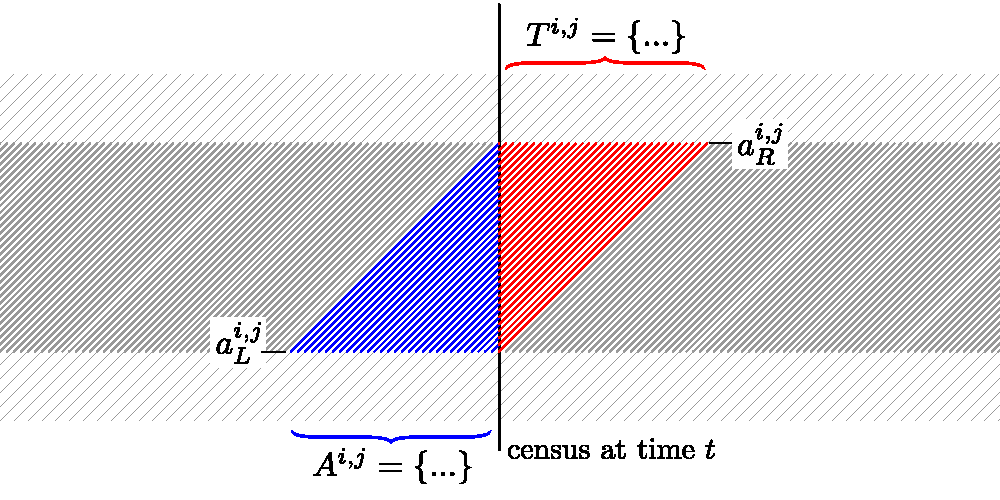
\includegraphics[scale=.8]{Figures/lifelinerepeated.pdf}
\end{figure}

Formally, sets $A^{i,j}$ and $T^{i,j}$ consist of the same values as the previous, but
coming from distinct instances of life trajectories generated in a uniform series from between $t-a_R^{i,j}$ years
ago until as recently as $t-a_L^{i,j}$ years ago. This demonstrates both
period-cohort set equality and time spent-left set equality. The blue and red triangles in
Figure~\ref{fig:clones} are simple rotations of one another.

\begin{tcolorbox}
Continuing with the episode $d^{21,1}$ in Tab.~\ref{tab:traj}, if we replicate this trajectory in single year steps, and take a census in year $t$, the values of $A^{21,1}$ and $T^{21,1}$ are the same as before $\{0,1,2\}$, but taken from three different life trajectories that began in years $t-4$, $t-3$, and $t-2$, and were observed at ages 3, 2, and 1, respectively.
\end{tcolorbox}
\FloatBarrier
\item{\textbf{Identical set concatenation identity:}} Repeat the construction of time spent and time left values for some other reference episode, $d^{i`,j`}$, as in step 1. This episode might have a different duration, their
sets of time-spent, $A^{i`,j`}$, and time left $T^{i`,j`}$ will be equal to one another but potentially distinct from those drawn from the previous trajectory-episode. $A^{i,j}$ and $T^{i,j}$ range from 0 to $d^{i,j}$, whereas $A^{i`,j`}$ and $T^{i`,j`}$
range from 0 to $d^{i`,j`}$. However, their concatenations are identical:

\begin{equation}
\label{eq:unioneq}
\{A^{i,j} , A^{i`,j`}\} = \{T^{i,j} , T^{i`,j`}\}
\end{equation}

The concatenation identity also applies if we replicate the life trajectory $d^{i`,j`}$ in $\delta$ time steps as in step 2. It is also true if we weight the sets derived from each trajectory by the probability of observing each trajectory.

\begin{tcolorbox}
For example, the \nth{22} trajectory from Tab.~\ref{tab:traj}, \vb{SSSH}, has a single episode of sickness of duration three, yielding identical sets with four observations $A^{22,1} = \{0,1,2,3 \}$ and $T^{22,1} = \{3,2,1,0 \}$. If the trajectory is replicated as in step 2, the observations of $d^{22,1}$ will come from four cohorts born in years $t-5$ through $t-1$ and captured at ages 3, 2, 1, and 0, respectively. Whether observed over time as in step 1 or over individuals within time, as in step 2, the concatenation of $A^{21,1}$ and $A^{22,1}$ is equal to the concatenation of $T^{21,1}$ and $T^{22,1}$, $\{0,0,1,1,2,2,3 \}$. If each birth cohort derived from the probabilities in Tab.~\ref{tab:toy} starts with 100000 individuals, once in stationarity we would expect a hypothetical census to yield 540$\times$4 instances of trajectory 21 and 60$\times$5 of 22, so we would expect 600 observations of values 0, 1, and 2, and 60 observations of 3 from these two unique paths. 
\end{tcolorbox}

\item{\textbf{Distribution equality by induction:}} By induction we can keep adding state episodes from the stationary population, constructing $A$ and $T$ for each, and concatenating over episodes as in step 3. The concatenation of all episode-specific time-spent sets and the concatenation 
of the corresponding time-left sets will always be identical. This is so both within trajectories and over time (cohort) and over trajectories observed at a single point in time (census). Therefore the probability of selecting a particular value from the concatenated time-spent set is identical
to the probability of selecting the same value from the cocnatenated time-left set, and Theorem~\ref{th} is proved.

\begin{tcolorbox}
To complete our worked example, the full expected distribution of time spent and left in episodes of sickness in a stationary series based on a renewal of 100000 individuals per year following the rates in Tab.~\ref{tab:toy} is shown in Fig.~\ref{fig:toydist}.
\end{tcolorbox}

 \begin{figure}[h!]
\centering
\caption{The symmetrical distribution of expected time spent and time left in sickness (\vb{S}) as of a census in the stationary population derived from the transition rates in Tab.~\ref{tab:toy} and 100000 individuals per birth cohort.}
\label{fig:toydist}
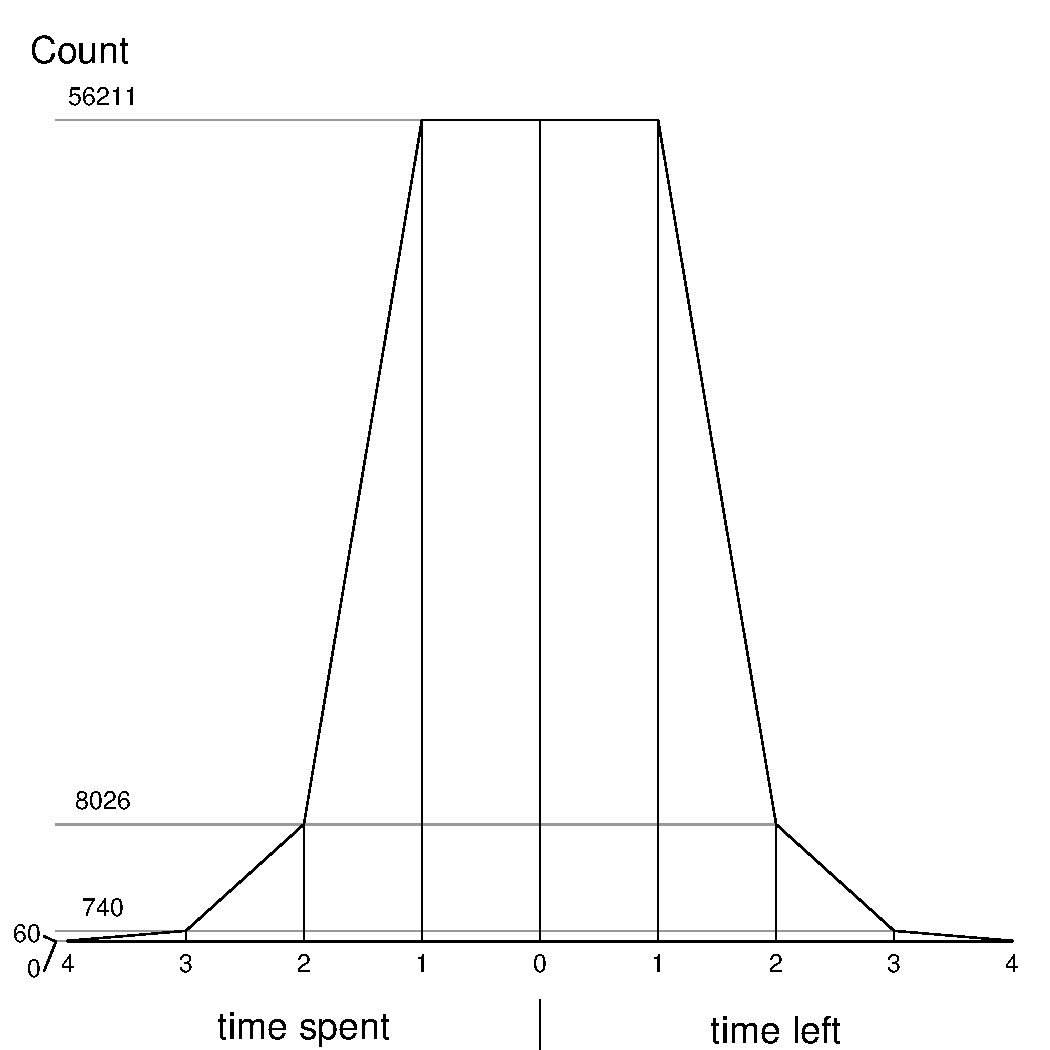
\includegraphics[scale=.5]{Figures/ToyDist.pdf}
\end{figure}

\end{enumerate}
\FloatBarrier
\end{proof}

\begin{proof}[Proof 2 of Theorem \ref{th}]
The second proof is in development.
\end{proof}

Our point of departure was that of a fixed discrete transition rates implying fixed probabilities of a finite number of discrete life trajectories, ultimately producing a stationary population with a fixed expected distribution of sampling paths, fixed expected age-state structure, and fixed expected age-state-episode duration structure.

\section{Discussion}
The approach from this proof is equally valid to prove the
original statement of the Brouard-Carey equality (where the state is ``alive''),
but it is more general.
The statement and proof is flexible enough to hold for irreversible and reversible
states. It also applies to repeatable states, whether time spent in the
state is kept in cumulative fashion over spells, or whether the clock resets to
zero on each entry into the state. The equality may also be conditionable in
curious ways: for example, the distribution of time-spent in a state conditional
on having entered at age $a$ must also be equal to the distribution of time-left in
the state, conditional on having entered at age $a$. Likewise, one may condition
statements on exit age. One may also arbitrarily merge states, and the equality
still holds within the newly merged state.

At first glance, this equality is probably less intuitive than the
original Brouard-Carey equality, because state entry is not necessarily aligned
on age zero. It is less visible in commonly-produced plots because plots of
stacked sequences look chaotic, often even if clustered or sorted. It might
be tempting to think that due to state-varying vital rates, the equality simply ought not hold.
However, the basis of the proof is the observation that if each individual
duration is symmetrical by complements, then so are aggregations of
durations, irrespective of alignment. Since each cohort in a perfectly
stationary population of infinite size is an identical copy of the previous,
census-like cross-sections are also equally-composed.

\section{Potential applications}
Empirical applications of the presently-described transient tenure equality may
be easy to conjure up. For example, imagine a hypothetical health state that
shows no noticeable symptoms, but that is medically measurable. One
may take a census with regular follow-ups, until eventually the state is exited
by each individual, whether by absorption into death or entry into another
state. Then, if the assumption of stationarity is acceptable, one may be able to
say something about onset timing in the aggregate, itself unobserved. %We think
%that the present equality will come as good news to researchers in similar
%settings.

\section{Simulation}
[section commented out until exercise more completely designed]
% The reader may wish to have a sense of how well this equality holds up under
% various violations of our assumptions. The assumption of invariant transitions
% is trickier to handle than that of finite populations with stochasticity. We
% conduct a simple markov chain simulation to
% produce random populations of different sizes derived from the same
% set of stationary transition probabilities. Our transition rates come
% from a published study of working life expectancy in older ages in the USA
% \citep{Dudel2017}, and refer to US black females around the year 1994. The transition matrix includes
% single ages 50-100, with lifetable closeout at age 100. Transient states include
% employed, unemployed, inactive, and retired. We generate random sequences of
% trajectories using the \texttt{rmarkovchain} function of the
% \texttt{markovchain} \texttt{R} package \citep{spedicato2017}.
% 
% For simplicity, all trajectories begin in a state of employment at age 50. We
% generate 1000, 10000, and 100000 individual trajectories. Out of these we
% sample observations of inactivity a total of 100, 1000, and 10000 times,
% respectively with replacement. We assume that the time of
% observation is half way through the year, but that spells begin on January 1 and
% end on December 31. For each observation of inactivity we measure the time spent
% in the spell up to the point of observation, and the time left until exiting the
% spell. These values are then tabulated for each simulation to produce
% distributions to compare. The theorem states that the distributions of time
% spent and left in this procedure should be asymptotically identical, but we have
% induced noise with the simulation, and we should be able to see distributions
% converge as simulated population and draw sizes increase.
% 
% 


\section{Conclusion}
Stationary populations are more symmetrical with respect to time lived and
spent than has been previously described. We have given an intuitive proof that
the distribution of time spent and left is equal within states in
stationary populations. We do not presume that this relationship will be immediately able to answer pressing questions, but we
hope that it may inspire new approaches in empirical measurements. We think
that that researchers working with left-censored or truncated data or
any kind of multistate models should be generally aware of this equality in case
it may come in handy as a heuristic.

The relationship between years lived
and left established by the Brouard-Carey equality is itself amenable to non-zero growth rates \citep{riffe2015renewal}.
We speculate that the transient tenure equality we describe here may also be tractable in stable
populations, but we have not investigated this possibility in detail. Future
research, potentially more sophisticated simulations, should establish the
impact of departures from stationarity and establish the fuzzy bounds of
usability for this relationship.



%\bibliographystyle{chicago}
\bibliographystyle{spbasic}
\bibliography{references}  
\end{document}
